\section{UC MVDR algorithm}
\label{sec:ucmvdr-algorithm}
The UC MVDR ABF projects the sample zeros radially on the
unit circle staying consistent with the unit circle constraint on the
ensemble MVDR polynomial zeros. By placing zeros on the unit circle,
the UC MVDR ABF guarantees beampattern nulls in the directions
corresponding to the unit circle zeros. The constraining approach used
by UC MVDR ABF is similar in spirit to ABF approaches which enforce
known structural constraints in the ensemble quantity onto the sampled
data based implementation, e.g., forcing Toeplitz structure when
evaluating the SCM in case of planewave beamforming using ULA
\cite{fuhrmann1991toeplitz}. The rest of the section describes the UC
MVDR algorithm assuming the beamformer is steered towards the
broadside ($\ulook = 0$). The algorithm extends naturally to the case
of a different look direction ($\ulook = u_L$) by rotating all the
zeros to match the look direction.

Algorithm~\ref{alg:ucmvdr} outlines the UC MVDR ABF
implementation. The algorithm begins from the SMI MVDR weights
$\wsmi$. The $z$-transform of the conjugated weights gives the SMI
MVDR polynomial $\smipoly(z) = \ztrans{(\wsmi\herm)}$. Factoring the SMI
MVDR polynomial in terms of the zeros,
\[
\smipoly(z) = G \prod\limits_{n=1}^{N-1}(1 - \sampz_n z\inv),  
\]
where $G$ is a scaling level to ensure unity gain in the look
direction ($\ulook = 0$), i.e., $\smipoly(\expo{j\pi\ulook}) = 1$ and $\sampz_n = r_ne^{j\omega_n}$ is the $n^{th}$ SMI MVDR
polynomial zero. As previously discussed in \sect{}\ref{sec:smi-poly},
the sample zeros are not necessarily on the unit circle
and hence the magnitudes $|\sampz_n| = r_n$ of the roots are generally
not unity. The next step is to radially project the SMI MVDR
polynomial zeros $\sampz_n$ to the unit circle. \figurename{}~\ref{fig:ucmvdr-cartoon} illustrates the projection of the sample zeros (diamond markers) to the unit circle where the zeros are denoted with circle markers. Projection yields a
set of unit circle zeros $\ucz_n = e^{j\omega_n}$ denoted by circle
markers. An exception occurs when the sample zeros fall within the CBF
main-lobe region in the complex plane
i.e. $|\operatorname{arg}(\sampz_n)|<2\pi/N$. Projecting such
zeros radially to the unit circle results in nulls inside the
main-lobe of the UC MVDR ABF. A null inside the main-lobe results in
an undesired effect of the main-lobe distortion and drastic loss in
WNG \cite[Sec.~6.3.1]{vtree2002oap}. Rather than radially projecting
to the unit circle, such zeros are moved to the closest CBF
first-null location on the unit circle such that
$\operatorname{arg}(\ucz_n) = \sign(\omega_n){2\pi/N}$ where
$\sign(\cdot)$ is the sign function. Keeping the zeros outside the
main-lobe region ensures the UC MVDR main-lobe remains undistorted.

\begin{figure}[!hp]
\centering
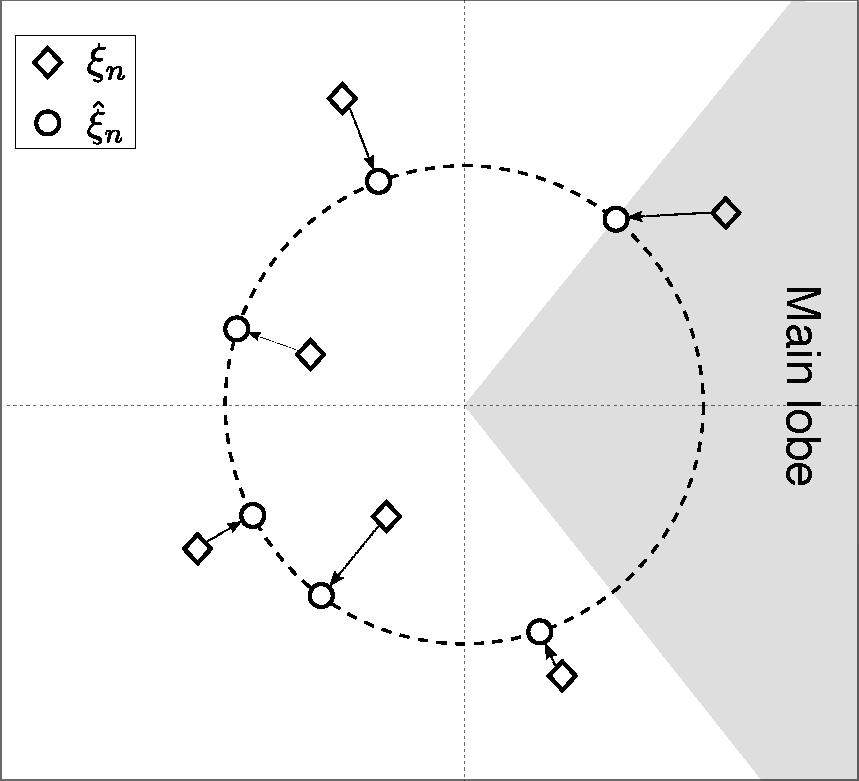
\includegraphics[width=0.9\textwidth]{ucmvdr_cartoon}  
\caption[Schematic shows the unit circle projection
technique.]{Schematic shows the unit circle projection technique. The
  diamond markers denote the sample zeros ($\sampz_n$) and the circle
  markers denote the unit circle zeros ($\ucz$) obtained by radially
  projecting the sample zeros. The sample zeros within the main-lobe
  region ($-2/N \leq u \leq 2/N$) are moved to the closest CBF
  first-null location ($u_{\text{null}} = \pm 2/N$) on the unit
  circle.}
\label{fig:ucmvdr-cartoon}
\end{figure}

The projected unit circle zeros $\ucz_n$ are used to synthesize a unit
circle polynomial
\begin{align}
\label{eq:uc-poly}
\ucpoly(z) =& \prod\limits_{n=1}^{N-1}\frac{(1 - \ucz_n z\inv)}{(1 - \ucz_n)}. \nonumber \\
\intertext{Rewriting the polynomial in terms of the coefficients
}
\ucpoly(z) =& \sum\limits_{n=0}^{N-1} c_n^* z\inv.
\end{align}
Comparing \eqref{eq:uc-poly} to the definition of the array polynomial
\eqref{eq:beampat-poly}, the coefficients $c_n$s can be viewed as
beamformer weights. Thus, the UC MVDR ABF weight vector is defined as
$\wuc = [c_1, c_2, \ldots, c_N]\trans$. Evaluating $\ucpoly(z)$ on the
unit circle produces the UC MVDR ABF beampattern with $N-1$ nulls in
the directions corresponding to $\ucz_n$s and a unity gain in the look
direction ($\ulook = 0$), i.e., $\ucpoly(\expo{j\pi\ulook}) = 1$.

\begin{algorithm}
  \caption{DZ MVDR beamformer} \label{alg:ucmvdr}
  \begin{algorithmic}
    \Procedure{SMI MVDR}{$\datavec{}$}\Comment{Compute SMI MVDR weights}
     \State $\sampCov = \frac{1}{L}\sum\limits_{\ell=1}^L\datavec\datavec\herm$
     \State $\wsmi = {\sampCov\inv\replook}/{(\replook\herm\sampCov\inv\replook)}$
    \EndProcedure
    \Procedure{ProjectUnitCcircle}{$\wsmi$}\Comment{Project zeros to unit circle}
    \State $\smipoly(z) = \ztrans (\wsmi\herm) = G\prod\limits_{n=1}^{N-1}(1 - \sampz_nz\inv)$ 
    \State  $\sampz_n = r_ne^{j\omega_n}$ \Comment{SMI MVDR polynomial zero}
     \If{$|\omega_n| > 2\pi/N$}
     \State $\ucz_n = e^{j\omega_n}$     
     \ElsIf{$|\omega_n| \leq 2\pi/N$}
     \State $\ucz_n = e^{\sign(\omega_n){j2\pi/N}}$
     \EndIf
     \EndProcedure
     \Procedure{UC MVDR}{$\ucz_n$}\Comment{Compute UC MVDR weights}
    \State $\ucpoly(z) = \prod_{n=1}^{N-1}(1 - \ucz_n z\inv)/(1 - \ucz_n) = \sum_{n=0}^{N-1} c_n^*z^{-n}$ 
    \State $\wuc = [c_1, c_2,\ldots,c_N]\trans$
    \EndProcedure
  \end{algorithmic}
\end{algorithm}

%  In order to satisfy the
% distortionless constraint of the MVDR beamformer, the $c_n$s are
% scaled to force unity gain in the look direction. The resulting UC
% MVDR beamformer weight vector is
% $\wuc = {\bf{c}}/{\replook\herm\bf{c}}$ where
% $\mathbf{c} = [c_0, c_1 \ldots c_{N-1}]$ and $\replook$ is the array
% manifold vector for the look direction $\ulook = \cos(\theta_0)$.
% Since the polynomial zeros are invariant to coefficient scaling, the
% UC MVDR beampattern still has nulls in the same locations as the
% polynomial $\ucpoly(z)$.

\figurename{} \ref{fig:smi-ucmvdr-plots} shows a representative
example comparing the UC MVDR and the
SMI MVDR ABF using an $N = 11$ sensor ULA and $L = 12$ snapshots. Both
ABFs are steered to broadside ($\ulook = 0$) look direction and a
single interferer is present at $\uinter = \cos(\theta_I) = 3/N$. In
\figurename{}~\ref{fig:smi-ucmvdr-pzplot}, the green diamond markers
indicate the SMI MVDR polynomial zero locations and the red circle
markers indicate the UC MVDR zeros projected on unit
circle. \figurename{}~\ref{fig:smi-ucmvdr-bpplot} shows nulls and
lowered sidelobes in the UC MVDR beampattern (solid red) in contrast
to the shallow notches and higher sidelobes of the SMI MVDR
beampattern (dot-dash green). The lowering of the sidelobes reduces
the area under the beampattern magnitude, which in turn improves the
WNG of the UC MVDR as described by \eqref{eq:wng-beampat}.

As discussed in \sect{}\ref{sec:smi-poly}, the SMI MVDR polynomial
zeros are randomly perturbed in both magnitude and phase from the
ensemble zero locations on the unit circle. Projecting the SMI MVDR
polynomial zeros back on the unit circle corrects the magnitude
perturbation in the sample zeros thereby satisfying the
unit circle constraint on the ensemble zeros. Moreover, the UC MVDR
weights can be seen as the closest approximation of SMI MVDR weights
in the ensemble constrained space, i.e., on the unit circle.

\begin{figure}[!hp]
\centering
\subfloat[Zero locations]
{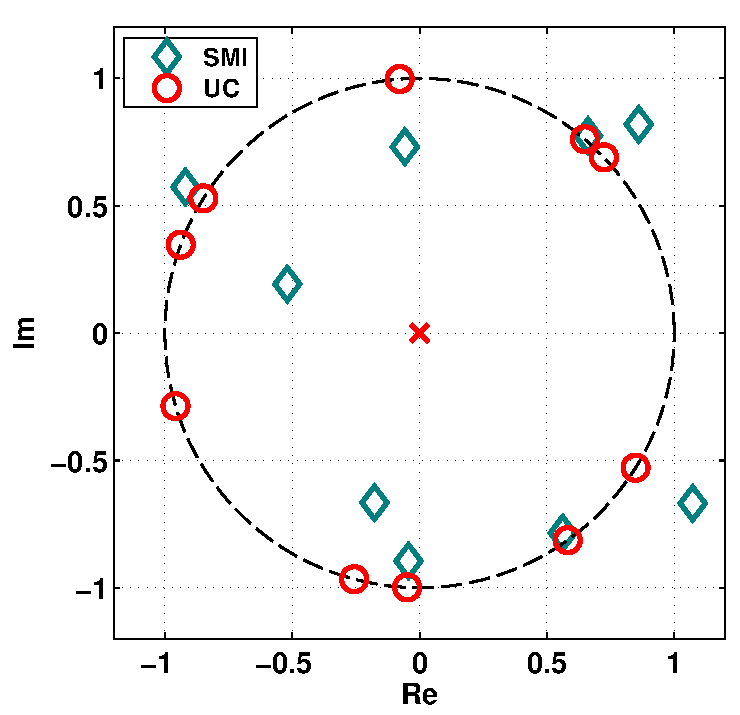
\includegraphics[width=3.5in]{mvdr_smi_dl_zfc_N11_pzplot_eg}  \label{fig:smi-ucmvdr-pzplot}}

\subfloat[Log-magnitude beampattern]{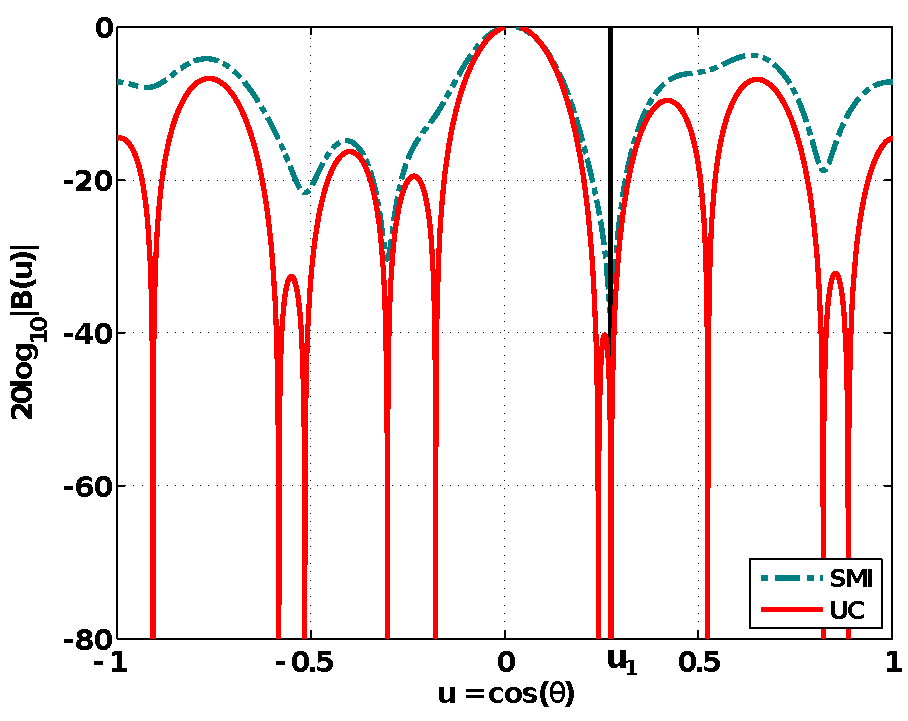
\includegraphics[width=3.5in]{mvdr_smi_dl_zfc_N11_bpplot_eg}  \label{fig:smi-ucmvdr-bpplot}}
\caption[Zero locations and log-magnitude beampatterns of a
representative example of the SMI MVDR and the UC MVDR ABF.] {Zero locations
  and log-magnitude beampatterns of a representative example of SMI
  MVDR (blue) and UC MVDR ABF (magenta) using $N = 11$ sensor ULA for
  $L = 12$ snapshots and look direction $\ulook = 0$. The unit circle
  zeros of the UC MVDR ABF produce nulls and lowers sidelobes compared
  to the SMI MVDR ABF beampattern.}
\label{fig:smi-ucmvdr-plots}
\end{figure}

%%% Local Variables: 
%%% mode: latex
%%% TeX-master: "main"
%%% End: 
